\chapter{Machine learning approach}
\label{ch:MachineLearning}
\graphicspath{{Chapter4/Chapter4Figures/}}
The previous chapter briefly described the basic workings of the optical mark recognition(OCR) system inside the automatic test grader. There is still one critical piece of information that has not been observed in the system. This information is the characters that the student writes into the designated boxes.

\nomenclature[dcnnAcronym]{$DCNN$}{Deep convolutional neural network}
This next chapter will provide two machine learning approaches to significantly improve the accuracy of the system over the previous standalone basic system. Firstly an approach to locate and classify hand written characters, provided by the students, using a deep convolutional neural network(DCNN), will be described. A more accurate method in determining the true digit represented by the bubble and character evidence, using a probabilistic  graphical model(PGM), will also be implemented. This PGM method will then allow for an integrated probabilistic approach to determine the true student number using the bubble as well as character evidence. It will be determined that the PGM is accurate enough to determine the student number by only using the character recognition information provided.

For a more detailed explanation on the DCNN used in this thesis, refer to Appendix \ref{sec:DCNN}.

\section{Character recognition using a neural network}

\subsection{Introduction}
\nomenclature[dcnnAcronym]{$ANN$}{Artificial neural network}

An neural network is a powerful machine learning tool for approximating complex functions. The basic architecture of a neural network can be seen in Figure \ref{fig:nn}. The structure of an feed-forward neural network consist of an input, hidden and output layer, as described in \citet{MichealN2015}. A artificial neural network(ANN) is a simplified approximation of how neurons in the brain works. Each neuron in the network acts as a small processing unit. The final output can thus be collected by reading the value at the output layer after it has been passed each layer of the network.

\begin{figure}
  \centering
  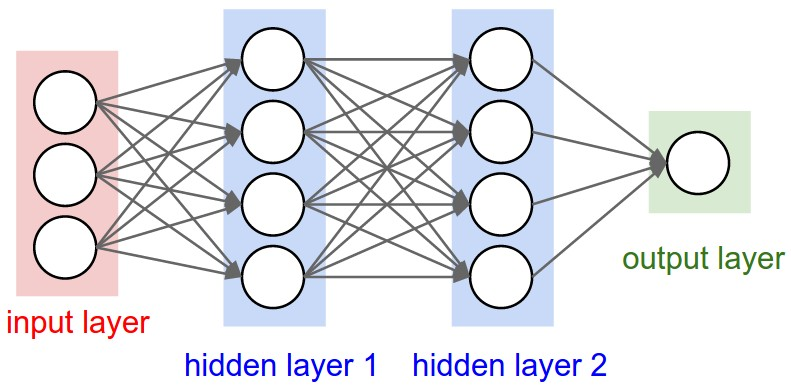
\includegraphics[width=14cm]{NN}\\
  \caption{Basic structure of an neural network, \citet{karpathy2017}}%, 
  \label{fig:nn}
\end{figure}

For this thesis a neural network will be trained to predict what digit, from 0 to 9, is most likely present in a image.  Figure \ref{fig:mnist} illustrates the input of of the neural network using and 14 by 14 example image. For this thesis a 28 by 28 greyscalled image will be used as input. Thus if each pixel represents one value, ranging from 0.0 to 1.0, there is total of 748 input values. 

\begin{figure}
  \centering
  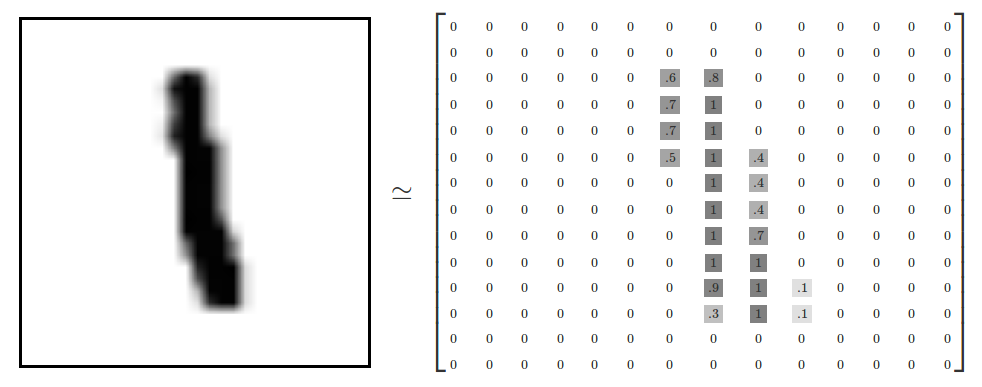
\includegraphics[width=14cm]{MNIST}\\
  \caption{Example image used as input to the neural network, \citet{tensor2017}}%, \citet{tensor2017}
  \label{fig:mnist}
\end{figure}

\subsection{Neural Network Basics}

\subsubsection{The artificial neuron}

The neuron unit takes in decimal values as input. The first step is then to calculate the weighted sum of these inputs, as shown in, Equation \ref{eqn:nnOut}.  Where $c$ is the number of inputs. $x_{i}$ and $w_{i}$ respectively are the input and weight values at index i. 

\begin{align}
% \nonumber to remove numbering (before each equation)
  z =  &\displaystyle{\sum_{i=0}^{c} x_{i}*w_{i}}
\label{eqn:nnOut}
\end{align}

The summed value then gets normalize using an sigmoid function, seen in Equation \ref{eqn:sigmoid}.

\begin{align}
  Out(z) =  &\displaystyle{\frac{1}{1 + e^{-z}}}
  %Out =  &\displaystyle{\sfrac{1}{4}}
\label{eqn:sigmoid}
\end{align}

This artificial neuron thus basically takes in a weighted input and produces a normalized out. By adjusting the weights, certain inputs will excite and others inhibit the output of the neuron more. This process thus allows different functions to be approximated by changing these weights. If a network of these neurons gets place together, shown in Figure \ref{fig:nn}, complex functions can be trained onto the network. These weights variables thus needs to be tuned to specific values, to allow the network to best categorize digits given an image. The process of calculating values for these weights will be covered in Section sec:trainNN.

\subsubsection{Getting a output from the network}

After the 748 input values have been assigned to the network inputs, each of the network's coulombs can be calculated one at a time. The first coulomb in the hidden layer will thus use the 748 input values and produce a normalize output for each of the neurons in that coulomb. This is done using using the previously mentioned equations \ref{eqn:nnOut} and \ref{eqn:sigmoid}. Once the first column's outputs are calculated the next column can be calculated. This process is repeated until all the columns are calculated in the hidden layer. The output layer is then calculated using the same method. For the character recognition in the test grader, 10 output neurons will be used, corresponding to the probability of the 10 digits being present. The values observed on the output neurons, gets normalized and used as the probability of each digit being present, using Equation  \ref{eqn:normal}. Where $prob(i)$ is the probability of digit $i$ being the character in the image. The value $Out(z_{i})$ us the output of the output neuron at index $i$.

\begin{align}
  prob(i) =  &\displaystyle{\frac{Out(z_{i})}{\sum_{k=0}^{10} Out(z_{k})}}
\label{eqn:normal}
\end{align}

\subsubsection{Training of neural network}
\label{sec:trainNN}

To train a neural network the MNIST dataset will be used. This is a database that has a labeled training set of 60,000 images, and a labeled test set of 10,000 images. The neural network will be trained using the training set. The basic idea behind the training method used in a neural network will be described in the following steps. For a more detailed description refer to Appendix \ref{ap:Algorithms}.

\begin{enumerate}
\item Calculate the network's output for each of the training images used in this training round.
\item Get the error margin of the network, using a formula that compares the true label of the training image, with the estimated label of the network.
\item Calculate the value with which each weight should be changed to reduce the error margin. One method of doing this is using the gradient decent with back propagation algorithms.
\item Repeat steps 1-3 until a time or accuracy criteria is met.
\end{enumerate}


\subsection{Preprocessing on image}
\label{sec:preprocess}

For the neural network to be able to classify digits from a 28 by 28 image, those subimages must first be found inside the test image. To do this Image processing is required. This is done in 6 steps as seen below: (Kry images by items om beter te lyk)

\begin{enumerate}
\item Find the contour closest to the expected location of the block, calculated in Section \ref{sec:findTemplate}. This is ilustrated in Figure \ref{fig:sa}. The bubbles have already been filter out of the image in a previous process.

\begin{figure}
  \centering
  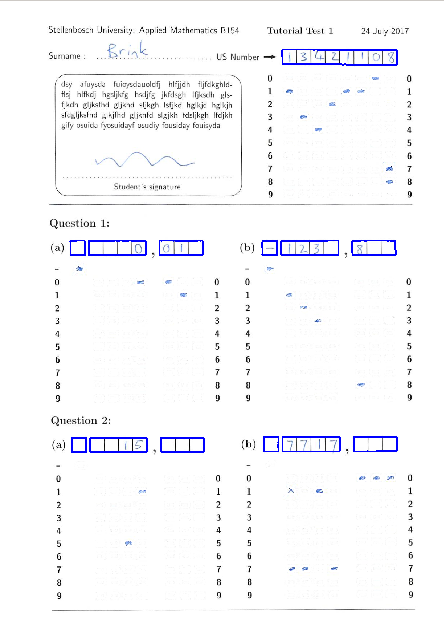
\includegraphics[width=8cm]{DigitScan}\\
  \caption{Image scanned for character areas.}
  \label{fig:sa}
\end{figure}

\item Transform the image to become fully rectangle using OpenCv's $four\_point\_transform$ method. This method applies a four point perspective transform on the image to reshape it into a rectangular form. An example of the final product can be seen in Figure \ref{fig:bp}.

\begin{figure}
  \centering
  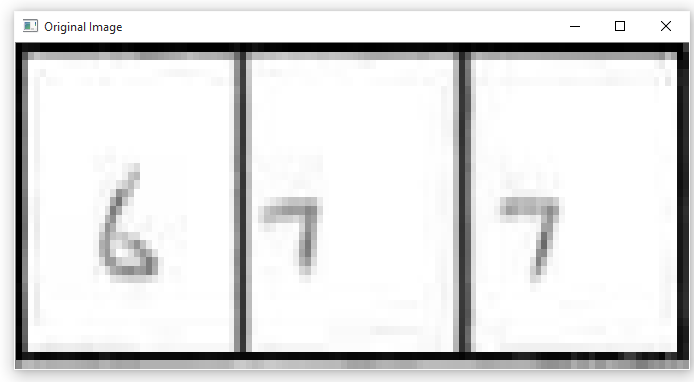
\includegraphics[width=10cm]{BeforeProcessing}\\
  \caption{The found box is then normalized to rectangular shape.}
  \label{fig:bp}
\end{figure}

\item Do a horizontal and vertical Radon transform, Section \ref{sec:RadonTransform}, to find and remove the dark box lines on the image, as seen in Figure \ref{fig:ar}.

\begin{figure}
  \centering
  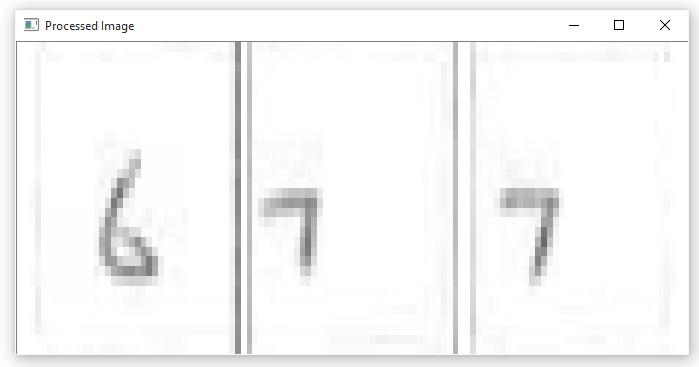
\includegraphics[width=10cm]{AfterRadon}\\
  \caption{a Randon transform then gets applied.}
  \label{fig:ar}
\end{figure}

\item Use the values received from the Radon transform to segment the image into the different boxes.
\item Using a custom segmentation algorithm, find the pixels most likely to belong to the digit, as seen in Figure \ref{fig:c}.

\begin{figure}
  \centering
  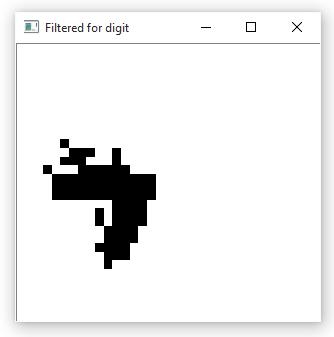
\includegraphics[width=4cm]{Cluster}\\
  \caption{An clustering algorithm is used to find the main cluster in the remaining image.}
  \label{fig:c}
\end{figure}

\item Locate the area the pixels are located in, as seen in Figure \ref{fig:areaLoc}

\begin{figure}
  \centering
  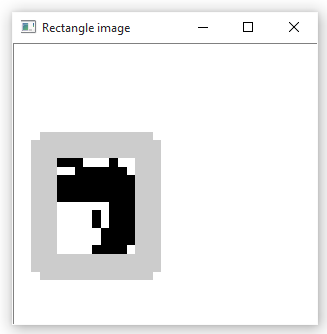
\includegraphics[width=4cm]{DetectArea}\\
  \caption{Area of found cluster.}
  \label{fig:areaLoc}
\end{figure}

\item Now calculate the center of the pixels, recenter and normalize the image area, as seen in Figure \ref{fig:final}

\begin{figure}
  \centering
  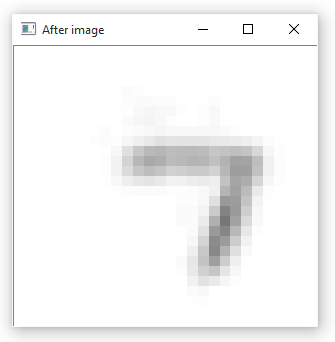
\includegraphics[width=4cm]{TranslateAndScale}\\
  \caption{Final translation and normalization of image.}
  \label{fig:final}
\end{figure}

\item Finally reshape the image into an 28 by 28 greyscalled image to be processed by the neural network.
\end{enumerate}

Each box on the image can now be classified by the neural network and  saved. The new character recognition evidence can now be used in combination with the bubble evidence to make a significantly more accurate estimate for the intended answers from the student. The next step is thus to combine all these individual evidence, in a intelligence way, to make a accurate prediction. A method to achieve this result will be covered in the next section.

\section{Probabilistic Graphical Models}
\label{sec:PGM}

The final step in determining the students answers is to probabilistic determining the most likely answers, given all the evidence presented. To do this a probabilistic graphical model(PGM) will be developed.

\subsection{Structure of the graph}

a Probabilistic graphical model(PGM) is a probabilistic graph containing random variables, where the graph expresses the conditional independence structure between these variables. The type of PGM used for this project is a Bayesian network. A Bayesian network models a set of random variables and their conditional dependencies via a directed acyclic graph (DAG). As seen in Figure \ref{fig:pgmDigit}, arrows are used to indicate which variables are conditionally dependent on another. 

The figure should be interpreted in the direction which information flows. Originally a student has a certain digit that he/she wants to portray on the page. This is given by the 'Digit user intended bubble'. There are 10 possible digits to consider and thus the bubble has 10 possible states. The intended digit gives rise to the intended bubbles and character that the student wants to write down. The student might sometimes mistakenly think that the first bubble represents 0 and thus even if the intended digit is 0 the intended bubble might be 1. Thus, this must also be done in a probabilistic manner to compensate for this uncertainty. The intended bubbles and character then produces evidence, as seen in Figure \ref{fig:pgmDigit}.  

When looking at Figure \ref{fig:column}, it is observed that there are 11 evidence areas to consider. They are the the 10 bubbles and the character block. The process of writing down this digit introduces so noise into the system, due to the fact the student is not always going to write down the digit in exactly the same way. Thus the evidence is also probabilistically linked to the 'intended bubble' and 'intended character' parent distribution. This evidence then gets written down on the paper and is what ultimately influences how the image looks. Each of the bubbles can take one of 4 states as evidence. These states are blank,crossed-out, partially colored in and fully colored in. The character block evidence is an 28 by 28 greyscale image. Thus it can have 28*28*256 possible states, where 256 is the possible pixel intensities of each pixel. This value with true range 0 to 256, gets converted into a normalized value between 0.0 and 1.0 when the neural network needs to process it.

\begin{figure}
  \centering
  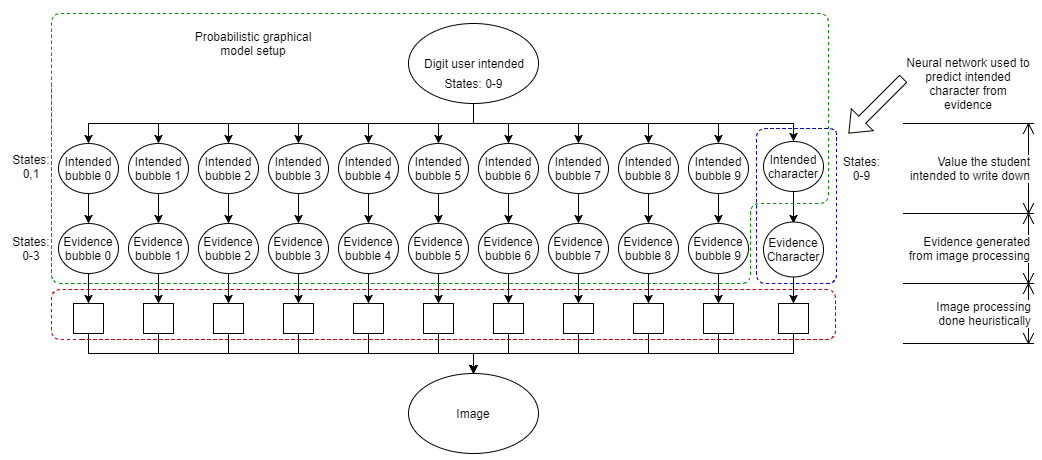
\includegraphics[width=16cm]{pgmDigit}\\
  \caption{Graphical setup of digit generation.}
  \label{fig:pgmDigit}
\end{figure}

\subsection{Determining the intended digit}
After the model is constructed the intended digit needs to be estimated, given the image. Thiss can be done by reasoning from the bottom(image evidence) upwards to the intended digit. The first step is to process the image that produces the evidence using of image processing. Producing the bubble evidence from the image is described in Chapter \ref{ch:ImageProcessing}. In \ref{sec:preprocess}, the process to extract the character evidence from the image was also described. Using the neural network the probability of intended character can be determined. After these steps have been completed the intended digit can be determined using the PGM, shown in Figure Figure \ref{fig:pgmDigit}. Thus is done by first setting the evidence node to the values calculated when image processing were done on them. The 'intended character' node then gets set to priors calculated through the use of the neural network. After this is done inference is done on the PGM and the resulting probability of each digit is calculated for the 'intended digit node'.

\begin{figure}
  \centering
  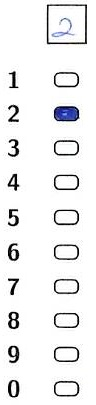
\includegraphics[width=1cm]{column}\\
  \caption{Column representing one digit.}
  \label{fig:column}
\end{figure}

\subsection{Training the model}

This subsection still needs to be completed.

As seen in Figure \ref{fig:pgmDigit},the PGM will include the bubble evidence as well as a prior probability that the neural network provides as evidence. Once these values are assigned, the PGM model will infer the intended digit using the probability distribution specified. To do this the conditional probabilities of the PGM, must first be determined from data. This is done by simple.. to be continued.


\subsection{Student number identification}
\label{sec:pgmStudentNum}
To be continued..
\section{Conclusion}

This chapter looked at two machine learning techniques to improve the accuracy with with the system infers the answers written on each scanned test sheet. A method was shown, using a neural network, to estimate the probability of each digit given only the character box as input. Additionally a approach was discussed, using a PGM, to allow the system to make a final prediction of what the student intended to write down given the bubble and character boxes as evidence.

The following chapter will cover the validation and results of the system from weekly grading done for the Applied mathematics department.